%%================================================
%% Filename: chap04.tex
%% Encoding: UTF-8
%% Author: 苏峻锋
%%================================================
\chapter{基于时间卷积网络的剩余性能的预测}
服务器集群运行时,由于访问时间,访问任务的不同,某些时间段整个集群可能处于忙碌的状态,某些节点可能处于任务繁忙任务重的而其他节点空闲的问题。
这样的两种节点是两种状态,高负载状态和低负载状态,处于低(高)负载状态的需要通过负载均衡器调整为正常负载状态,可以提高集群的总体资源利用率,环节高负 载节点的压力。
因此本章通过对于时间卷积网络的研究,针对某一个节点的剩余性能的预测,使得对服务器节点的负载分配进行均衡的调整。本文通过对普遍的 Linux 进行研究来获取相关数据。
\section{服务器剩余性能的获取}
动态负载均衡算法的负载性能会受到服务器负载指标选取的影响。选择合适的负载信息生成合适的负载指标能够真实的反映服务器运行是的负载情况,
提升算法的准确度和动态负载均衡的负载效果。在第二章中已经知道了有哪些负载信息值得挑选和收集,但是没有一个真正的合适的负载综合指标来体现真实的负载情况。
具体的剩余性能的获取可以使用 Linux 的 proc 文件系统获取,该文件储存在内存里,不会占用外存的空间。

(1)CPU 信息的获取 

要获取 Linux 系统中的 CPU 详细使用情况可以使用 cat/proc/stat,CPU 详细使用情况如下表。

\begin{longtblr}[
  caption = {CPU 详细信息解释},
]{
  width = \linewidth,
  colspec = {Q[102]Q[837]},
  vline{2} = {-}{},
  hline{1,9} = {-}{0.08em},
  hline{2} = {-}{},
}
参数      & 解释                                   \\
user    & 系统从启动到当前时刻,用户态 CPU 时间,不含 nice 值为负的进程 \\
nice    & 系统从启动到当前时刻,nice 值为负的进程占用的 CPU 时间     \\
system  & 系统从启动到当前时刻,核心时间                      \\
idle    & 系统从启动到当前时刻,除硬盘等待外其他等待时间              \\
iowait  & 系统从启动到当前时刻,硬盘等待时间                    \\
irq     & 系统从启动到当前时刻,硬中断时间                     \\
softirq & 系统从启动到当前时刻,软中断时间                     
\end{longtblr}

那么 CPU 利用率的计算公式为:$CPU_{usg} = 1 - (idle_2 - idle_1) / (cpu_2 - cpu_1)$ 通过使用 cat /proc/cpuinfo 命令获取服务器 CPU 配置,然后在 benchmark 上可纯到该 CPU 性能的分数作为 $CPU_{mark}$。则一个节点的 CPU 的剩余性能如下。
\begin{align}
  C_{j}=(1-CPU_{usg_{j}})\frac{n^{\ast}CPU_{mark_{j}}}{\sum_{1}^{n}CPU_{mark}}
\end{align}

(2) 内存信息获取
获取内存使用情况则可以 cat /proc/meminfo 命令,其中最重要的是 MemFree、Buffers、Cached 三个信息分别是完全空闲的内存大小、缓存文件系统的元数据和跟踪正在读写的块设备、存储页缓存和slabs的内存大小。所以内存使用率的计算方式如下。
\begin{equation}
  MEM_{usg} = (1 - MemFree + Buffers + Cached) / MemFree
\end{equation}

(3)磁盘信息获取

磁盘信息可以通过 iostat -x /dev/sda1  命令获取。重要信息如下表。

% \usepackage{tabularray}
\begin{longtblr}[
  caption = {磁盘信息获取},
]{
  width = \linewidth,
  colspec = {Q[81]Q[860]},
  hlines,
  vlines,
  hline{1,8} = {-}{0.08em},
}
标示~     & 说明                                                 \\
Device~ & 监测设备名称                                             \\
rkB/s~  & 每秒实际读取的大小,单位为KB                                    \\
wkB/s~  & 每秒实际写入的大小,单位为KB                                    \\
await~  & 等待I/O平均的时间(milliseconds)                           \\
svctm~  & I/O需求完成的平均时间                                       \\
\%util~ & 设备带宽的使用率,达到100\%表示饱和,达到性能瓶颈,如果是支持处理并发请求的设备则不代表性能瓶颈 
\end{longtblr}

(4)网络带宽信息获取

获取网络带宽使用 cat /proc/net/dev 命令,统计一段时间内 Receive 和 Tramsmit 的 bytes 值变化,可以获取网口传输速率 $T_{bytes}$,而网络带宽为 Bandwidth,则带宽利用率为:$NET_{usg} = T_{bytes} / Bandwidth$

获取了这几个重要的剩余性能的指标之后,也需要有一个能够体现综合负载情况的评价指标。为了以一种数学方法客观的计算出服务器节点当前的负载量,需要改造一个综合负载决策来组合各项负载指标。
常见的指标组合形式有加权和法和加权乘法,通过阅读不同的文献可知,在构建服务器负载状态的数学模型中,加权和法具有不错的效果\cite{lixbhunj}。在以往的负载均衡策略研究中这些权重系数通常依靠经验赋值确定,缺乏必要的数学分析和定量依据,为了使得服务器的计算结果更加准确和可靠,本文选取了主成分分析法科学计算综合负载决策函数的权系数向量。

主成分分析法(Principal Componet Analysis, PCA)最早是由 Pearson\cite{kpfrs1901lines}提出的一种多元统计方法,
该方法通过正交变换将原始数据转换成一组由线性无关变量变量表示的数据,以达到数据降维的目的\cite{李可佳2023基于主成分分析和函数机制的差分隐私线性回归算法}。具体步骤如下。

已经收集了服务器节点的 CPU 利用率、内存利用率、设备 IO 使用率,和带宽使用率的数据,将这些数据保存在以个表中,每一列代表一个指标,每一行代表一个观测时间点的数据。
由于主成分分析法的要求,将不同的特征量纲统一到相同的尺度,这样就可以公平地比较和组合这些特征,需要对给定数据集进行标准化。
对于每个指标,计算所有数据点的均值。公式为:$\mu=\frac{1}{N}\sum_{i=1}^{N}x_{i}$ 其中$\mu$ 为均值,N 是观测的个数,$x_{i}$ 每个观测的值。
计算标准差:然后计算每个指标的标准差。公式为:$\sigma = \sqrt{\frac{1}{N} \sum_{i = 1}^{N} \left(\right. x_{i} - \mu \left(\left.\right)\right)^{2}\frac{\sigma}{2}}$其中$\sigma$是标准差。
最后进行Z-score标准化:对每个指标的每个数据点进行标准化,公式为 $z = \frac{(x_{i} - \mu)}{\sigma}$ 其中 $z$ 就是最后每个指标每个观测时间的标准化后的值。

给定标准化后的数据集 $X = [x_1, x_2, \cdots, x_n]^{\mathbf{T}} \in \mathbb{R}^{n \times d}$,其中 $n$ 为样本的数量,$d$ 指标的数量,
结合在一起,\( X \) 是一个由 \( n \) 个 \( d \)-维的实数向量构成的数据集,并且以矩阵形式表示,其中每一行是一个样本,每一列是一个特征。则数据集的协方差公式矩阵如下。
\begin{equation}
  A={\frac{1}{n}}X^{\mathsf{T}}X={\frac{1}{n}}\sum_{i\,=\,1}^{n}x_{i}x_{i}^{\mathsf{T}}=V\Sigma V^{\mathsf{T}}\in\mathbb{R}^{d\cdot d}
\end{equation}

对 $\mathbf{A}$ 进行特征分解后得到一组降序排列的特征值$\lambda_1 \ge \lambda_2 ... \ge \lambda_n > 0$ 相对应的单位特征向量 $v_1, v_2, \dots, v_n$。
其中,特征值越大的,其对应的主成分越重要。于是,综合负载决策函数如下。
\begin{equation}
  \mathbf{X} = 1000 \times (\mu_1C_{usg} + \mu_2M_{usg} + \mu_3D_{usg} + \mu_4N_{usg})
\end{equation}

通过指定欲保留的主成分比重阈值 $\theta \in (0, 1]$ 来确定目标唯独 k 的大小。
具体来说$\k$可以通过 $\frac{\sum^{k}_{i = 1}\lambda_i}{\sum^{d}_{i = 1}\lambda_i} \ge \theta$ 来得到。
取前 $k$ 个特征值对应的特征向量组成的主成分空间$\mathbb{V}_{d \times k} = (v_1, v_2, \cdots, v_k)$。将标准化后的原始数据集$\mathbf{X}_{n \times d}$ 投影到由前 $k$ 个特征向量构成的主成分空间 $\mathbf{V}_{d \times k}$中,得到了降维后的 $k$ 维数据集。
\begin{equation}
  \mathbf{Z}_{n \times k} = \mathbf{X}_{n \times d}\mathbf{V}_{d \times k}
\end{equation}
其中在进行特征分解后,就已经得到了主成分空间,空间内含有了最重要的4个特征值,
这个特征值就是权重的系数,通过降维与原始数据值相乘后得到的就是每个指标乘以权重系数后的数据集,只需要对降维的数据集进行每一列的相加,即可对得到时间序列-综合负载指标的数据集。

\section{时间卷积网络的关键特征}
时间卷积网络由传统的 CNN 改进的专门处理时间序列的深度学习模型\cite{lea2016temporal}。一开始认为,时序问题(如语言、语音等等)天生就是 RNN 的地盘。然而现在这一观点要成为过去式了。时间卷积网络(Temporal Convolutional Nets, TCNs)作为 CNN 家族中的一员健将,拥有许多新特性,如今已经在诸多主要应用领域中击败了 RNN。看起来 RNN 可能要成为历史了。

卷积神经网络(Convolutional Neural Nets, CNNs)是图像和视频识别领域公认的主力军,
而循环神经网络(Recurrent Neural Nets, RNNs)在自然语言处理领域的地位与其是相似的。
但二者的一个主要不同是,CNN 可以识别静态图像(或以帧分割的视频)中的特征,
而 RNN 在文本和语音方面表现出色,因为这类问题属于序列或时间依赖问题。
也就是说,待预测的后一个字符或单词依赖于前面的(从左到右)字符或单词,因此引入时间的概念,
进而考虑到序列。实际上,RNN 在所有的序列问题上都有良好表现,包括语音 / 文本识别、机器翻译、手写体识别、序列数据分析(预测),
甚至不同配置下的自动编码生成等等。但是它的问题是极度地计算密集,因为在整个任务运行完成之前,必须保存所有的中间结果,深度神经网络必须等前一个单词处理完,才能进行下一个单词的处理,于是 TCN 便应运而生。

时间卷积网络需要的数据集和RNN 有一定的类似,在处理时间序列数据集时都要进行嵌入(Embedding)操作。Embedding的主要目的是将时序数据映射到一个稠密的连续向量空间中,使得相似的语义信息在该向量空间中也能够彼此接近。这样,神经网络就可以基于这些向量表示学习到输入数据的复杂语义信息,并在相似的向量表示之间进行泛化。图是具体的嵌入过程。

\begin{figure}[htbp]
  \centering
  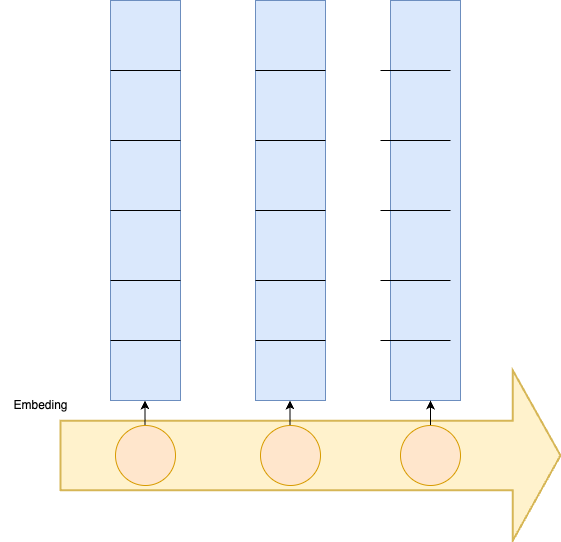
\includegraphics[width=0.7\textwidth]{figures/embedding.drawio.png}
  \caption{原始时序序列嵌入生成向量}
\end{figure}

TCN所依赖的卷积操作在本质上就是一维卷积(1D-CNN)。一维卷积利用多个大小固定的卷积核与输入序列进行卷积运算来生成输出序列。卷积核的形状由输入通道数$in\_channels$ 和卷积核大小$kernel\_size$ 共同决定,卷积核的数量则由输出通道数$out\_channels$决定。
经过Embedding后的时序数据的通道数由1扩展成了$embedding\_size$ ,对于有着 $in\_channels$ 个通道的时序数据作为输入, 一维卷积使用 $out\_channels$ 个大小为($in\_channels, kernel\_size$)的卷积核进行卷积操作。

假设有一个时间序列,总共有五个时间点,比方说股市,有一个股票的价格波动:[10,13,12,14,15]。TCN 使用一个卷积大小为 2 的卷积核,对上面5个数据做一个卷积核大小为2的卷积是什么样子如下。

\begin{figure}[htbp]
  \centering
  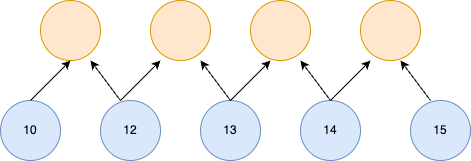
\includegraphics[width=.9\textwidth]{figures/convolution_1.drawio.png}
  \caption{卷积核为2的卷积过程}
\end{figure}

五个数据经过一次卷积,可以变成四个数据,
但是每一个卷积后的数据都是基于两个原始数据得到的,所以说,目前卷积的视野域是2。可以看到是输入是5个数据,但是经过卷积,变成4个数据了。TCN网络的第一个原则是输入和输出的形状必须相同。而在进行一维卷积操作时,假设第$i$ 层的输入长度为$L_i$ 卷积核大小为 $K$ 则输出长度为 $L_{i+1} = L_{i} - K + 1$。为满足这个原则,TCN在使用卷积神经网络进行序列处理时,通常需要进行 Padding 操作。通过在输入序列的左侧添加一定数量$K-1$ 的 0,实现信号维度的保持,使通过卷积和池化处理后的数据与输入数据的长度相同。在一维卷积中进行的Padding操作默认会在左右都进行填充,
所以TCN进行了额外的裁剪操作。

\begin{figure}[htbp]
  \centering
  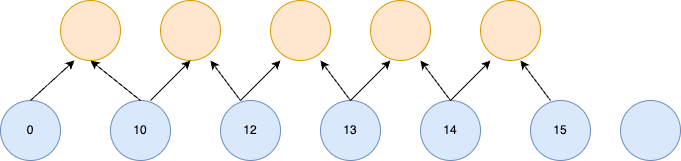
\includegraphics[width=0.9\textwidth]{figures/convolution_2.drawio.png}
  \caption{padding 后的卷积}
\end{figure}

padding是左右两头都增加0,如果padding是1的话,就是上图的效果,其实会产生6个新数据,但是秉着:“输入输出尺寸相同”和“我们不能知道未来的数据”,所以最后边那个未来的padding,就省略掉了,之后会在代码中会体现出来。

时间卷积网络有两个原则,其一就是上面的TCN 网络的输入和输出形状必须相同,以确保模型对时序数据的处理不会丢失信息。其二,TCN 网络中的每一时刻的输出仅由该时刻及其之前的输入卷积得到,以确保其在处理序列时具有因果约束。
通过使用因果卷积满足原则二,因果卷积是一种只考虑过去时间状态的一维卷积操作。因果卷积的具体步骤如下图所示。

\begin{figure}[htbp]
  \centering
  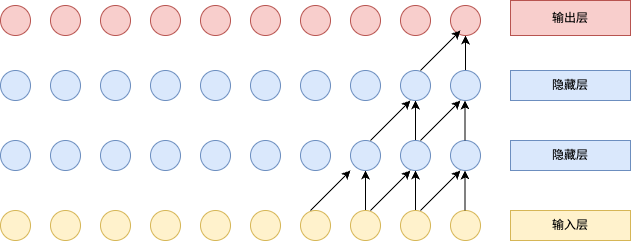
\includegraphics[width=\textwidth]{figures/causal_convolution.drawio.png}
  \caption{因果卷积}
\end{figure}

图中可以看到,因果卷积具备了两个特点。只考虑过去的信息。 时刻的输出$y_t$ 仅依赖于 $x_0,...,x_t$ ,而不依赖任何“未来”的输入$x_{t+1},...,x_T$。
同时追溯历史信息越久远,隐藏层越多。 图中,输出层期望采集输入层的4个时间步,则需要2个隐藏层。而业务的需求往往要求采取更多的时间步,确实是“深度”学习了。

由于因果卷积没有循环连接,它们通常比循环神经网络(RNN)训练速度更快,尤其是应用于非常长的序列。
但是,针对于一般的时间序列而言,往往是按照分钟记录的,那少说也是十万、百万的数据量,想要考虑之前1000个时间点呢?视野域要是1000,那意味着要999层卷积。
每经过一层,节点相对于前层减少一个,我们最后的输出只有一个节点,如果输入视野为1000,需要经过999层才能变为最后输出的一个节点。
啥计算机吃得消这样的计算。所以引入了膨胀因果卷积。

单纯的因果卷积还是存在传统卷积神经网络的问题,即对时间的建模长度是受限于卷积核大小的,如果要想抓去更长的依赖关系,就需要线性的堆叠很多的层。
标准的 CNN 可以通过增加 pooling 层来获得更大的感受野,而经过 pooling 层后肯定存在信息损失的问题。

膨胀卷积是在标准的卷积里注入空洞,以此来增加感受野。
和传统卷积不同的是,膨胀卷积允许卷积时的输入存在间隔采样,采样率受超参数 dilation rate控制,
指的是做卷积操作时kernel里面的元素之间的下标间隔。空洞的好处是不做 pooling 损失信息的情况下,增加了感受野,让每个卷积输出都包含较大范围的信息。下图就是 dilation=2 的时候的膨胀因果卷积的情况,

\begin{figure}[htbp]
  \centering
  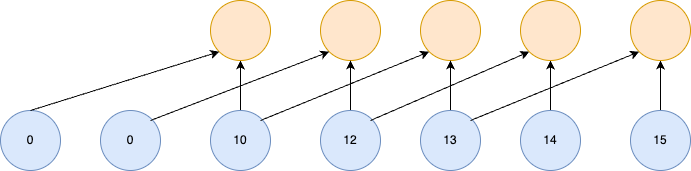
\includegraphics[width=\textwidth]{figures/dilation_convolution.drawio.png}
  \caption{dilation=1 的膨胀因果卷积}
\end{figure}

图中,可以看到卷积核大小依然是2,但是卷积核之间变得空洞了,每2个点采样一个作为输入;
如果dilation=3的话,那么可以想而知,这个卷积核中间会空的更大,每3个点采样一个作为输入。
因为dilation变大了,所以相应的padding的数量从1变成了2,所以为了保证输入输出的特征维度相同,
padding的数值在卷积核是2的情况下等于dalition的数值。
一般情况下,$padding=(kernel_size-1)\times dilation$,每个卷积核元素之间有 $dilation - 1$ 个空洞节点,
所以空洞因果卷积的感受野范围大小为 $(kernel_size-1) \times dilation + 1$。
以输入中的第一个元素作为空洞因果卷积的最后一个元素,则它的左边需要padding的个数为$(kernel_size-1) \times dilation$。于是较为完备的 TCN 训练网络如下。

\begin{figure}[htbp]
  \centering
  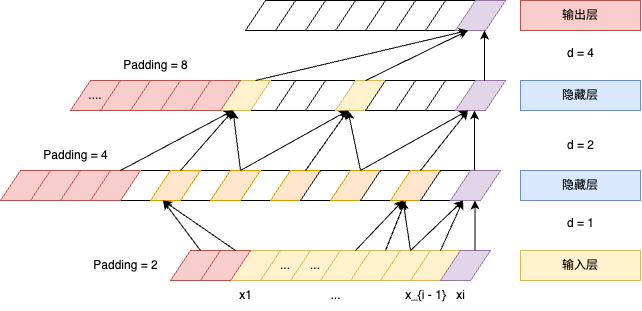
\includegraphics[width=\textwidth]{figures/tcn_1.drawio.png}
  \caption{TCN 训练网络骨干}
\end{figure}

从图中可以看到,每一层$t$ 时刻的值只依赖于上一层 $t, t - 1, \dots$ 时刻的值,体现了因果卷积的原则。而每一层对上一层信息的提取,都是跳跃式的,且逐层 dilated rate 以 2 的指数增长,体现了空洞卷积的特性。同时由于采用了空洞卷积,因此每一个隐藏层都需要做 padding,padding 的大小为 $padding = (kernel_size - 1)$。

在 CNN 中能够提取不同的特征,网络层数越多,意味着能够提取到不同等级的特征,并且,越深的网络提取的特征越抽象,越具有深层次的信息。但是如果简单的增加深度,就会导致梯度消失或者梯度爆炸。对于这个问题可以使用权重参数初始化和正则化层,这样可以训练几十层的网络\cite{吕国豪2014基于卷积神经网络的正则化方法}。
虽然解决了梯度消失的问题,但是网络退化出现了。高层次的神经网络空间虽然包含了低层次的网络空间,但是由于在训练中使用的是随机梯度下降策略,往往得到的是局部最优解,而不是全局最优解。

假设已经有了一个最优的网络结构,是 18 层。当设计网络结构时,并不知道具体多少层的网络拥有最优的网络结构,
假设设计了 34 层的网络结构。那么多出来的 16 层其实是冗余的,希望训练网络的过程中,模型能够自己训练这 16 层为恒等映射,也就是经过这16 层时的输入与输出完全一样。
但是往往模型很难将这 16 层恒等映射的参数学习正确,这样的网络一定比最优的 18 层网络表现差,这就是随着网络加深,模型退化的原因。
因此解决网络退化的问题,就是解决如何让网络的冗余层产生恒等映射即深层网络等价于一个浅层网络。

为了解决网络退化问题,残差模块应运而生,同时终结图片识别大赛。下面是一个残差模块的结构。

\begin{figure}[htbp]
  \centering
  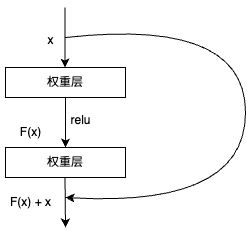
\includegraphics[width=0.5\textwidth]{figures/residual_block.drawio.png}
  \caption{残差模块}
  \label{residual_block}
\end{figure}

通常情况下让某一层网络学习恒等映射函数 $H(x) = x$ 比较困难,但是如果把网络函数设置为 $H(x) = F(x) + x$就可以吧恒等映射函数转化为一个残差函数 $F(x) = H(x) - x$,只要 $F(x) = 0$,就构成了一个恒等映射 $H(x) = x$。图\ref{residual_block}中,
iden mapping 被称为 shortcut 连接,residual mapping 即是 F(x)。残差的网络思想,如果网络已经到达最优,继续加深网络,residual mapping 将被 push 为 0,只剩下 identity mapping,这样理论上网络一直处于最优状态了,网络的性能也就不会随着深度增加而降低了。

实验证明,残差模块往往需要两层以上,单单一层的残差模块 并不能起到提升作用\cite{he2016deep}。shortcut 连接有两种,如果是同等维度的映射则 $F(x)=W_2σ(W_1x+b_1)+b_2,H(x)=F(x)+x$,
如果维度不同则 $F(x)=W_2σ(W_1x+b_1)+b_2,H(x)=F(x)+W_sx$。虽然残差模块刚开始是基于全连接层的表示,实际上残差模块可以用于卷积层。加法变为 channel 间的两个 feature map 逐个元素相加。下图\ref{residual_tcn}是时间卷积网络的残差模块。

\begin{figure}[htbp]
  \centering
  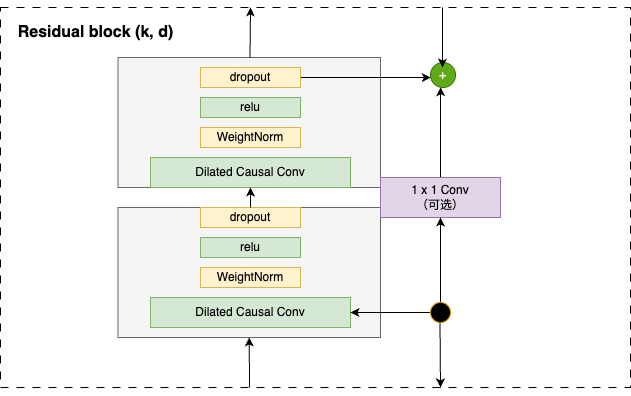
\includegraphics[width=\textwidth]{figures/resiual_tcn.drawio.png}
  \caption{TCN 的残差模块设计}
  \label{residual_tcn}
\end{figure}

于是整体的思路已经清晰,首先对时序数据集进行嵌入,嵌入使用指定大小的卷积核设置指定的膨胀因数,开始进行训练,进行归一向量化,和 ReLU 激活函数 Dropout 池化来防止梯度爆炸,最后用一个 Resnet 残差连接来避免梯度消失。

\section{时间卷积网络与负载情况的结合}
得到了综合负载评价指标和对应的时间就形成了一个常规的时间序列数据集,通过时间卷积网络深度学习即可较好的学习到时间序列内蕴藏的信息,通过蕴藏的信息预测未来的综合负载情况,返回给Nginx 集群内的负载均衡器,其以此来分配不同的不同的任务给空闲的服务器。

综合相关文献,对比了常规 RNN、LSTM、GRU 与 TCN 等循环神经网络在多种典型序列模型预测问题的性能表现上,结果表明 TCN 通常可以获得更好的预测精度,可以作为时间序列预测建模的有效手段\cite{bai2018empirical}\cite{赵洋2022基于时间卷积网络的短期电力负荷预测}。

(1)TCN 参数设置
由膨胀因果卷积的原理可知,TCN 模型中的扩大因子$d$ 和卷积核大小 $K$ 是决定TCN 模型预测性能的主要参数。此参数的选择目前尚无理论指导, 一般均需通过实验对比取得\cite{hewage2020temporal}。由于实验数据以及实验环境的限制,无法通过实验来确定当前不同配置的TCN模型的 $MAE$ 值和 $RMSE$ 值来确定最佳参数。但是可以列举几个比较通用的模型参数,其中, 扩大因子 d 分别取值为 2、4 、8 和 16 ;卷积核 K 分别取为 1×3、1×5 和 1×7 ,两组参数共构成 12 种组合形式,如下表所示。

% \usepackage{tabularray}
\begin{longtblr}[
  caption = {TCN 模型参数组合},
]{
  width = \linewidth,
  colspec = {Q[177]Q[158]Q[165]Q[183]Q[158]Q[160]},
  vline{4} = {-}{},
  vline{4} = {2}{-}{},
  hline{1,8} = {-}{0.08em},
}
序号 & \$d\$ & \$K\$ & 序号 & \$d\$ & \$K\$ \\
1  & 2     & 1x3   & 7  & 8     & 1x3   \\
2  & 2     & 1x5   & 8  & 8     & 1x5   \\
3  & 2     & 1x7   & 9  & 8     & 1x7   \\
4  & 4     & 1x3   & 10 & 16    & 1x3   \\
5  & 4     & 1x5   & 11 & 16    & 1x5   \\
6  & 4     & 1x7   & 12 & 16    & 1x7   
\end{longtblr}

通过使用不同参数的 TCN 模型可以得到 MAE(平均绝对误差)即观测值与预测值绝对差的平均值、RMSE(均方根误差)即观测值与预测值差的平方的平均值的平方根。来确定最佳参数。 通过指定训练参数 epoch 以及 lr 来获得预测值,在通过与观测值的比较即可选择到较好的模型参数。

\section{本章总结}

本章首先探讨了如何获取到剩余性能的数据,并根据科学的主成分分析法来选取合适的权重参数,用合适的权重参数得到了能较好体现负载情况的综合负载指标数据集。

接着讨论了时间卷积网络与其他循环神经网络的不同之处,得到了其在时间序列预测性能的特征和具体原理和具体过程。最后将综合负载指标已经对应的时间戳形成对应的时间序列数据集。通过设置 epoch 和 lr 来暂时确定 MAE 和 RMSE 的走势情况,以获取训练的最佳参数。
设置了最佳参数后可以进行更大的 epoch 来实现更好的预测性能。
